\documentclass[14pt]{beamer}
\usetheme{Pittsburgh}
\usepackage{xcolor}
\definecolor{USUBlue}{RGB}{26,57,89}
\usecolortheme[named=USUBlue]{structure}
\setbeamercolor{normal text}{fg=USUBlue}
\usepackage[utf8]{inputenc}
\usepackage{mathptmx}
\usepackage{tgbonum}
\usepackage{amssymb}
\usepackage{graphicx}
\usepackage{marvosym}
\usefonttheme{structuresmallcapsserif}
\usefonttheme{serif}
\setbeamercolor{author}{fg=USUBlue}
\setbeamerfont{author}{size=\small}
\setbeamerfont{frametitle}{size=\large}
\setbeamertemplate{enumerate items}[default]
\author{Elita Baldridge\\ @elitabaldridge}
\title[17pt]{A data-intensive assessment of the species-abundance distribution.}
\setbeamertemplate{navigation symbols}{}
\date{}
%\setbeamercovered{transparent} 
%\logo{\includegraphics[scale=.03]{../Miscellaneous/Pictures/ecology_center_horizontal.jpg}\includegraphics[scale=0.07]{../Miscellaneous/Pictures/Weecology.png}} 
\institute{\includegraphics[scale=.07]{../Miscellaneous/Pictures/ecology_center_horizontal.jpg}\includegraphics[scale=0.35]{./sad-data/dissertation/WeecologyProduction.png}} 
%\subject{} 

\begin{document}

\section{Usage Notes}
\begin{frame}[t]
\frametitle{A data-intensive assessment of the species-abundance distribution.}
\begin{large}
Feel free to:\\
\end{large}
\includegraphics[scale=.5]{./sad-data/dissertation/use.png}\\
\begin{large}
Provided that:\\
\end{large}
\includegraphics[scale=.5]{./sad-data/dissertation/attribution.png}
\end{frame}

\section{Title}
\begin{frame}[t]
\titlepage
\end{frame}

%\begin{frame}
%\tableofcontents
%\end{frame}

\section{Introduction}
\subsection{Let's begin with an example..}
\begin{frame}
\frametitle{Let's begin with an example...}
\begin{center}
\includegraphics[scale=.4]{./sad-data/dissertation/BeetleRAD.png}\\
\end{center}
\end{frame}

\begin{frame}
\frametitle{Let's begin with an example...}
\begin{center}
\includegraphics[scale=.4]{./sad-data/dissertation/BeetleRAD_w_graph.png}\\
\end{center}
\end{frame}


\begin{frame}
\frametitle{Pattern \& process.}
\note{
Few common species.
Many rare species.
One of the most fundamental and ubiquitous patterns in ecology.}
Species abundance distribution (SAD)
\begin{itemize}
\item Reveals pattern-generating mechanisms of community structure.
\end{itemize}
\begin{center}
\includegraphics[scale=.4]{./sad-data/dissertation/realistic_even_RAD.png}\\
\end{center}
\note{
Few common species.
Many rare species.
One of the most fundamental and ubiquitous patterns in ecology.
Species abundance distribution (SAD)
\begin{itemize}
\item Describes the distribution of commonness \& rarity of species.
\end{itemize}
\begin{center}
\includegraphics[scale=.4]{./sad-data/dissertation/generichollowcurves.png}\\
\end{center}
\begin{itemize}
\item Many potential pattern-generating mechanisms.
\item Exhibits a hollow curve distribution.
\end{itemize}
Relative abundance distribution (RAD)
Species abundance distribution (SAD)}
\end{frame}


\begin{frame}
\frametitle{Pattern \& process.}
\begin{center}
\includegraphics[scale=.35]{./sad-data/dissertation/PatternProcess_example_text.png}\\
\end{center}
\end{frame}


\begin{frame}
\frametitle{Patterns \& process.}
\begin{Large}
\begin{center}
Process\\ 
\includegraphics[scale=.35]{./sad-data/dissertation/ProcessesPattern.png}\\
Pattern\\
\end{center}
\end{Large}
\end{frame}

\subsection{What is macroecology?}
\begin{frame}[t]
\frametitle{Macroecology}
\normalsize One approach for identifying general ecological patterns \& processes.
\begin{center}
\includegraphics[scale=.30]{./sad-data/dissertation/SpatialTaxonomic.png}
\end{center}
\note{
\begin{itemize}
\item Data intensive.
\item Large scales.
\end{itemize}
\begin{itemize}
\item Spatial
\item Temporal
\item Taxonomic
\end{itemize}
\begin{itemize}
\item Search for general patterns \& processes.
\end{itemize}}
\end{frame}


\begin{frame}[t]
\frametitle{Traditional approach}
\vspace{-7pt}
\begin{center}
\includegraphics[scale=.45]{./sad-data/dissertation/localclose.png}
\end{center}
\end{frame}


\begin{frame}[t]
\frametitle{Broader approach}
\vspace{-7pt}
\begin{center}
\includegraphics[scale=.45]{./sad-data/dissertation/birdmapclose.png}
\end{center}
\end{frame}

%\subsection{Commonness & rarity}
%\begin{frame}[t]
%\frametitle{Commonness \& rarity}
%"Who can explain why one species ranges widely, and is very numerous, and why another %allied species has a narrow range and is rare?  Yet these relations are of the highest %important, for they determine the present welfare and, as I believe, the future success %and modification of every inhabitant of this world."\\ 
%~\\ 
%Darwin, 1859.\\
%\end{frame}

\begin{frame}
\frametitle{Pattern \& Process;\\ Signal \& Noise}
\begin{center}
\includegraphics[scale=.4]{./sad-data/dissertation/SignalNoise.png}
\end{center}
\note{
\begin{Huge}
\begin{center}
Pattern\\ 
\MVArrowDown{}\\  
Process\\  
\MVArrowDown{}\\
Prediction
\end{center}
\end{Huge}}
\end{frame}

%\subsection{Challenges of macroecology}
%\begin{frame}[t]
%\frametitle{Challenges of macroecology}
%\begin{itemize}
%\item Studies performed with a limited number of large datasets.
%\item Lack of identification of pattern generating mechanisms.
%\end{itemize}
%\note{
%Taxonomic and ecosystem limitations in datasets, e.g.North American terrestrial bias.}
%\end{frame}

%\subsection{Best practices}
%\begin{frame}[t]
%\frametitle{Best practice recommendations}
%\begin{itemize}
%\item Test multiple models with consistent statistical approach.
%\item Test with multiple taxonomic groups/ecosystems.  
%\end{itemize}
%\vspace{-7pt}
%\begin{center}
%\includegraphics[scale=.2]{./sad-data/dissertation/SpatialTaxonomic.png}
%\end{center}
%\end{frame}

\section{Outline}
\begin{frame}
\frametitle{Data-intensive ecology}
\begin{itemize}
\item Leveraging existing ecological data.
\item The species abundance distribution.
\item The statistical approach.
\item The mechanistic approach.
\end{itemize}
\end{frame}


\section{Leveraging existing ecological data}
\subsection{Current Data}
\begin{frame}[t]
\frametitle{Current Data}
\vspace{-7pt}
\begin{center}
\includegraphics[scale=.45]{./sad-data/dissertation/ExistingDataMap.png}
\end{center}
\note{
\begin{large}
Major macroecological datasets\\
\end{large}
\begin{itemize}
\item Largely terrestrial
\item Largely North American
\item Many publicly available, some not.
\end{itemize}
~\\
~\\
~\\
~\\
\begin{large}
Lots of data in the literature.\\
\end{large}}
\end{frame}


\subsection{Compiled Data}
\begin{frame}[t]
\frametitle{Macroecological data}
Challenges of macroecology\\
\begin{small}
\begin{itemize}
\item Lack of identification of process.
\end{itemize}
\end{small}
Best practice recommendations
\begin{small}
\begin{itemize}
\item Test with multiple taxonomic groups/ecosystems. 
\end{itemize}
\end{small} 
\begin{large}
~\\
Plenty of data in the literature.
\end{large}
\end{frame}


\subsubsection{Introduction to Ecoinformatics}
\begin{frame}[t]
\frametitle{The Rules of Ecoinformatics}
\begin{Large}
Garbage in, garbage out.\\
\end{Large}
\begin{itemize}
\item All data are good, not all data are appropriate.
\item Fit the data to the question.
\end{itemize}
\end{frame}

\begin{frame}[t]{}
\frametitle{Building a database}
\note{
\begin{itemize}
\item Decide on inclusion criteria.
\item Decide what variables to collect.
\item Decide on handling of missing data.
\item Decide on database structure.
\item Search for data.
\item Sort papers into useable and not.
\item Collect data.
\end{itemize}}
\begin{center}
Record decisions at all steps:\\
~\\
\begin{large}
\emph{Metadata are important.}
\end{large}
\end{center}
\end{frame}


\subsubsection{Data Collection}
\begin{frame}[t]{}
\frametitle{Abundance database}
Inclusion criteria:
\begin{itemize}
\item Quantitative abundances (counts).
\item Complete sampling.
\item Raw data (not heavily processed).
\item Observational.
\end{itemize}
\end{frame}

\begin{frame}[shrink=30]
\frametitle{Abundance database}
\begin{table}
\begin{tabular}{l} 
 Variables collected\\ 
\hline
\\
 Class \\
 Family\\
 Genus \\
 Species (Specific epithet)\\
 Abundance \\
 Collection Year, starting\\
 Collection Year, ending \\
 Site Name \\
 Biogeographic region \\
 Site notes\\
 Citation\\ 
\end{tabular}
\caption{List of variables collected.}
\end{table}
\end{frame}

\subsubsection{Data Wrangling}
\begin{frame}[t]
\frametitle{Data wrangling}
\begin{center}
\includegraphics[scale=.37]{./sad-data/dissertation/WranglingRaw.png}
\end{center}
\end{frame}

\begin{frame}[t]
\frametitle{Data wrangling}
\begin{center}
\includegraphics[scale=.32]{./sad-data/dissertation/WranglingEntry.png}
\end{center}
\end{frame}

\begin{frame}[t]
\frametitle{Data wrangling}
\begin{center}
\includegraphics[scale=.32]{./sad-data/dissertation/WranglingEnd.png}
\end{center}
\end{frame}

\subsubsection{Data Summary}
\begin{frame}{}
\frametitle{Abundance database}
\includegraphics[scale=.35]{../Miscellaneous/Pictures/Phd/CompiledData.png}
\end{frame}

\begin{frame}{}
\frametitle{Abundance database}
\includegraphics[scale=.27]{./sad-data/dissertation/bioregions.png}
\end{frame}

\begin{frame}{}
\frametitle{Abundance database}
\includegraphics[scale=.45]{./sad-data/dissertation/taxa_sites.png}
\end{frame}

\subsubsection{Data Availability}
\begin{frame}[fragile]
\frametitle{Data Availability}
~\\
~\\
Public \& open access through figshare.\\
EcoData Retriever importable.\\
\begin{verbatim}
(http://figshare.com)
(http://www.ecodataretriever.org)
sad_data = 
ecoretriever::fetch('MiscAbundanceDB')
\end{verbatim}
\includegraphics[scale=.3]{./sad-data/dissertation/retriever_logo_wtext.png}
\includegraphics[scale=.5]{./sad-data/dissertation/figshare_FullColour.jpg}
\end{frame}

\subsection{Analysis Data}
\begin{frame}{}
\frametitle{Data}
\begin{center}
\includegraphics[scale=.4]{./sad-data/dissertation/Database.png}
\end{center}
\end{frame}


\begin{frame}{}
\frametitle{Data}
\includegraphics[scale=.4]{./sad-data/dissertation/AllDatasets.png}
\end{frame}

\begin{frame}[shrink=35]
\frametitle{SAD Comparisons}
\begin{center}
\begin{table}
\begin{tabular}{l|c|l|r}
 Dataset &Dataset code &Availability &Sites\\
\hline
 Gentry's Forest Transects &Gentry &Public &10355\\
 Breeding Bird Survey &BBS &Public &2769\\
 Christmas Bird Count &CBC &Private &1999\\
 Forest Inventory Analysis &FIA	 &Public &220\\
 N. American Butterfly Count &NABA &Private &400\\
 Actinopterygii, compiled &Actinopterygii &Public &161\\
 Reptilia, compiled &Reptilia &Public &138\\
 Mammal Community Database &MCDB &Public &103\\
 Amphibia, compiled &Amphibia &Public &43\\
 Arachnida, compiled &Arachnida &Public &25\\
 Coleoptera, compiled &Coleoptera &Public &5\\
\end{tabular}
\caption{Datasets used for species-abundance distribution comparisons. Datasets marked as Private obtained through data requests to the providers with Memorandums of Understanding.}
\end{table}
\end{center}
\end{frame}

\section{The species abundance distribution}
\subsection{Pattern description}
\begin{frame}[t]{}
\frametitle{Commonness \& rarity}
~\\
\begin{large}
The species abundance distribution:
\end{large}
\begin{center}
\includegraphics[scale=.52]{./sad-data/dissertation/genericRAD.png}\\
\end{center}
\note{
\begin{itemize}
\item Describes the distribution of commonness \& rarity of species.
\item One of the most fundamental and ubiquitous patterns in ecology.
\item Exhibits a hollow curve distribution.
\begin{itemize}
\item Many rare species.
\item Few common species.
~\\
\end{itemize}
\end{itemize}}
Many models of the species abundance distribution (SAD).
\end{frame}

\subsection{Forms of the distribution}
\begin{frame}[t]
\frametitle{SAD models}
Statistical description\\
\begin{center}  
\includegraphics[scale=.2]{./sad-data/dissertation/Preston1948.png}
\begin{tiny}
Preston 1962a.\\
\end{tiny}
\end{center}
Process-based\\
\begin{center}
\includegraphics[scale=.25]{./sad-data/dissertation/Rosindelletal2011.png}
\begin{tiny}
Rosindell et al. 2011.\\
\end{tiny}
\end{center}
\end{frame}
 

\section{SAD comparisons: The statistical approach.}
\begin{frame}
\frametitle{SAD comparisons: The statistical approach.}
\begin{large}
Most comparisons of the different models:
\end{large}
\begin{itemize}
\item Use a small subset of available models (typically two).
\item Focus on a single ecosystem or taxonomic group
\item Fail to use most appropriate statistical methods. 
\end{itemize}
\end{frame}

\subsection{Data & Analysis}
\begin{frame}
\frametitle{SAD Comparisons}
\begin{center}
\includegraphics[scale=.35]{./sad-data/dissertation/SpatialTaxonomic.png}
\end{center}
\end{frame}

\subsubsection{Model selection}
\begin{frame}[shrink=10]
\frametitle{SAD Comparisons}
~\\
~\\
Selected five models from four classes for comparison.
\begin{table}
\begin{tabular}{l|l}
 Model class & Form of the distribution\\ 
\hline
 Purely statistical & Logseries, Poisson lognormal\\
 Branching process & Zipf \\
 Population dynamics & Negative binomial\\
 Niche partitioning & Geometric \\
\end{tabular}
~\\
~\\
~\\
~\\
\caption{After B.J. McGill et al. 2007.}
\end{table}
\end{frame}

\subsubsection{Analysis}
\begin{frame}[t]
\frametitle{SAD Comparisons}
~\\
Analysis:
\begin{itemize}
\item Model fitting with maximum likelihood estimation.\\
\begin{itemize}
\item For a given model, estimates model parameters that provide the most likely characterization of the data.
\item Best practice for fitting species abundance distributions. \begin{tiny} Matthews \& Whittaker 2014.\end{tiny}
\end{itemize}
~\\
%$l_x(\theta) = \log h(x) + \log f_\theta(x)$
\end{itemize}
\end{frame} 


\begin{frame}[t]
\frametitle{SAD Comparisons}
~\\
Analysis:
\begin{itemize}
\item Likelihood based model selection to compare the fits of the different models.
\begin{itemize}
\item How well does the model describe the data?
\end{itemize}
\end{itemize}
\end{frame}

\begin{frame}[t]
\frametitle{SAD Comparisons}
~\\
Analysis:
\begin{itemize}
\item Model comparison with corrected Aikaike Information Criterion (AICc) weights.
\begin{itemize}
\item How well does the model describe the data relative to the number of parameters?
\end{itemize}
\item The best fitting model had the greatest AICc weight. 
\end{itemize}
\end{frame}

\begin{frame}
\frametitle{SAD Comparisons}
~\\
Computational tools:
\begin{itemize}
\item Model fitting, log-likelihood, \& AICc: macroecotools Python package.\\
\begin{small}
(https://github.com/weecology/macroecotools)
\end{small}
\item All code \& majority of data are publicly available.
\begin{small}
(https://github.com/weecology/sad-comparison)
\end{small}
\end{itemize}
\begin{center}
\includegraphics[scale=.40]{./sad-data/dissertation/GitHub-Mark-120px-plus.png}
\end{center}
\end{frame}

%\begin{frame}
%\frametitle{Open science}
%\begin{Large}
%More reproducible.\\
%More accessible.\\
%~\\
%\begin{huge}
%\emph{Better science.}
%~\\
%~\\
%\end{huge}
%\end{Large}
%\begin{center}
%\includegraphics[scale=.2]{./sad-data/dissertation/Open_Access.png}  
%\includegraphics[scale=.15]{./sad-data/dissertation/osi_logo.png}
%\end{center}
%\end{frame}


\subsection{Results}
\begin{frame}{}
\frametitle{SAD Comparisons}
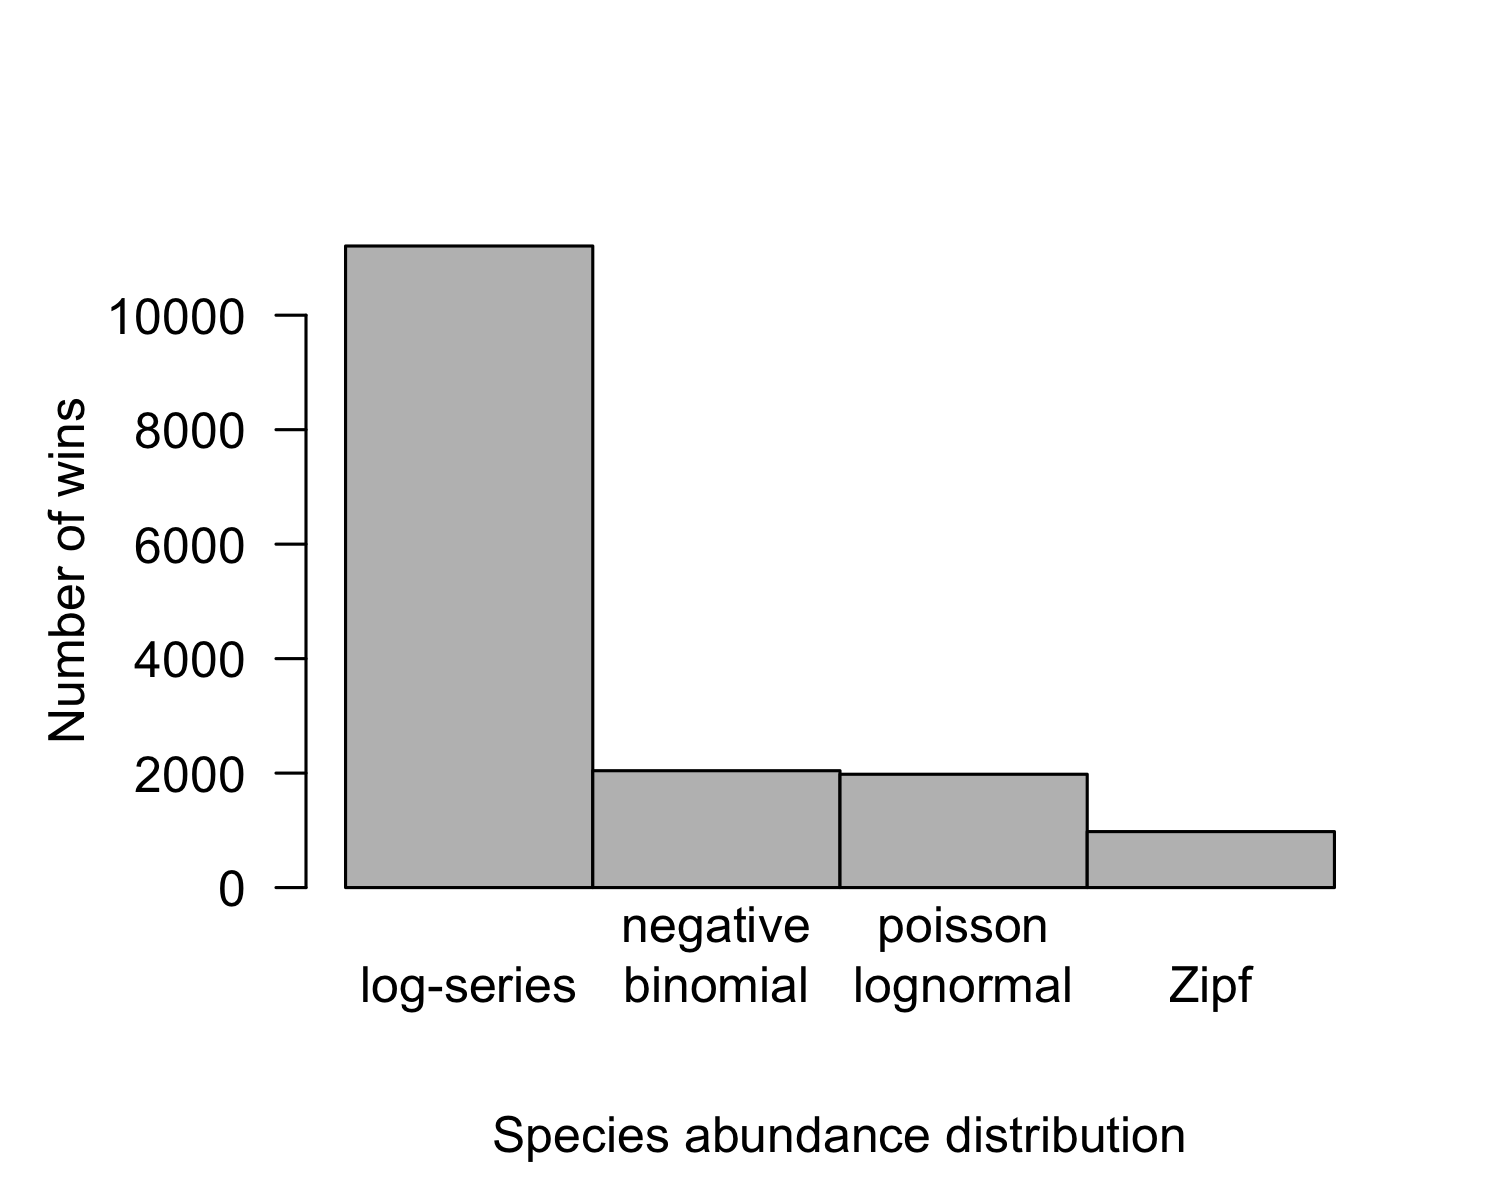
\includegraphics[scale=.5]{./sad-data/dissertation/total_wins.png}
\end{frame}

\begin{frame}{}
\frametitle{SAD Comparisons}
\includegraphics[scale=.40]{./sad-data/dissertation/wins_by_dataset.png}
\end{frame}

\begin{frame}{}
\frametitle{SAD Comparisons}
\includegraphics[scale=.5]{./sad-data/chapter1/Zipf_weights.png}
\end{frame}


\begin{frame}{}
\frametitle{SAD Comparisons}
\includegraphics[scale=.5]{./sad-data/dissertation/AICc_weights.png}
\end{frame}

\begin{frame}{}
\frametitle{SAD Comparisons}
\includegraphics[scale=.5]{./sad-data/dissertation/likelihoods.png}
\end{frame}

\begin{frame}{}
\frametitle{SAD Comparisons}
\includegraphics[scale= 1]{./sad-data/dissertation/Zipf_one_to_one.png}
\end{frame}

\begin{frame}{}
\frametitle{SAD Comparisons}
\includegraphics[scale=.43]{./sad-data/dissertation/likelihoods_one_to_one.png}
\end{frame}

\subsection{Conclusions}
\begin{frame}
\frametitle{SAD Comparisons}
Existing models provide equivalently good absolute fits to empirical data.
\begin{itemize}
\item Models with fewer parameters perform better in AIC-based model selection.\\
\item Logseries provides a good naive model for fitting SADs.\\
\note{
\begin{itemize}
\item Produces equivalent likelihoods.
\item Has a single fitted parameter.
\item Easy to fit to empirical data.
\item Best overall model.
\end{itemize}}
\end{itemize}
\end{frame}

\begin{frame}[t]
\frametitle{Identifying process:}
\vspace{-7pt}
\begin{center}
\includegraphics[scale=.3]{./sad-data/dissertation/SpatialTaxonomic.png}
\end{center}
\begin{itemize}
\item Examine scale dependence of pattern.
\item More general approach to process?
\end{itemize}
\end{frame}

\section{The mechanistic approach: Neutral analysis.}
\subsection{Neutral & non-neutral processes}
\begin{frame}[t]
\frametitle{Neutral processes}
~\\
Many formulations of neutral theory, but:
~\\
\begin{itemize}
\item Species \& individuals ecologically \& demographically equivalent.\\
\end{itemize}
\includegraphics[scale=.35]{./sad-data/dissertation/Rosindelletal2011.png}\\
\begin{tiny}
Rosindell et al. 2011.
\end{tiny}
\note{
\begin{itemize}
\item Species \& individuals ecologically \& demographically equivalent.\\
\item Stochastic variation in birth, death, immigration, \& speciation results in species abundance differences.
\end{itemize}}
\end{frame}

\begin{frame}[t]
\frametitle{Non-neutral processes}
\begin{center}
\includegraphics[scale=.4]{./sad-data/dissertation/non-neutral-processes.png}\\
\end{center}
Many specific mechanisms, but:
~\\
\begin{itemize}
\item Shape of the abundance distribution due to differences among species.\\
\end{itemize}
\end{frame}

\subsection{Neutral Analysis}
\begin{frame}
\frametitle{The mechanistic approach: Neutral analysis.}
Early tests of neutral theory compared the fit of empirical species abundance distributions to the neutral prediction.\\
~\\
Later tests suggested species abundance comparisons were insufficient for a rigorous test of neutrality.\\
~\\
\begin{Large}
\emph{However...}
\end{Large}
\end{frame}

\begin{frame}
\frametitle{Neutral Analysis}
Connolly et al. 2014 simulated neutral communities.\\
\begin{center}
\includegraphics[scale=.4]{./sad-data/dissertation/Connolly2014A.png}
\end{center}
\note{
\begin{small}
\begin{itemize}
\item Compared model fits of a non-neutral distribution (Poisson lognormal) to a neutral distribution (negative binomial distribution).\\
\item Distinct abundance values a measure of power related to the number of species in a community to fit models.
\end{itemize}
\end{small}}
Identified a signal of neutrality.\\
\end{frame}

\begin{frame}
\frametitle{Neutral Analysis}
Connolly et al. 2014 identified non-neutral species abundance distributions in marine communities.\\
\begin{center}
\includegraphics[scale=.4]{./sad-data/dissertation/Connolly2014B.png}
\end{center}
\note{
\begin{small}
\begin{itemize}
\item Compared model fits of a non-neutral distribution (Poisson lognormal) to a neutral distribution (negative binomial distribution).\\
\end{itemize}
\end{small}}
May be a robust method for identifying communities that exhibit non-neutrality.\\
Untested in terrestrial systems.
\end{frame}


\subsection{Data & Analysis}
\begin{frame}
\frametitle{Neutral Analysis}
\frametitle{SAD Comparisons}
\begin{center}
\includegraphics[scale=.2]{./sad-data/dissertation/SpatialTaxonomic.png}
\end{center}
Used the same data and model fitting approach.\\
\end{frame}

\begin{frame}{}
\frametitle{Neutral Analysis}
Non-neutral model (Poisson lognormal)\\
\begin{itemize}
\item Describes communities generated by non-neutral processes.
\end{itemize}
Neutral model (negative binomial).\\
\begin{itemize}
\item Describes communities generated by neutral processes.
\end{itemize}
\end{frame}

\begin{frame}{}
\frametitle{Neutral Analysis}
\includegraphics[scale=.43]{./sad-data/dissertation/EmpirModelHist.png}
\end{frame}

\begin{frame}{}
\frametitle{Neutral Analysis}
\begin{center}
\includegraphics[scale=.43]{./sad-data/dissertation/Connolly2014B.png}
\end{center}
\begin{tiny}
Connolly et al. 2014.
\end{tiny}
\end{frame}


\subsection{Results}
\begin{frame}{}
\frametitle{Neutral Analysis}
\includegraphics[scale=.40]{./sad-data/dissertation/avgvals_by_dataset.png}
\end{frame}

\begin{frame}{}
\frametitle{Neutral Analysis}
\includegraphics[scale=.45]{./sad-data/dissertation/distabclasses_vs_lognormwgt.png}
\end{frame}

\subsection{Conclusions}
\begin{frame}
\frametitle{Neutral analysis}
Difficult to identify a clear winning model.
\begin{itemize}
\item Demonstrates the importance of testing with multiple ecosystems.
\end{itemize}
\end{frame}

\section{General Conclusions}
\begin{frame}{}
~\\ 
\frametitle{A data-intensive approach}\
Challenging to infer process from species abundance distributions alone.
~\\ 
\begin{itemize}
\item Broad model categorization (i.e. neutral or non-neutral) may be more productive.
\item May not be one single suite of processes that dominates.
\end{itemize} 
\end{frame}

\begin{frame}[t]{}
\frametitle{A data-intensive approach}\
~\\ 
Challenges in identifying mechanism among datasets.
~\\ 
\begin{itemize}
\item Biological vs. non-biological differences (spatial structuring, sampling intensity).
\item Diverse data removes uncertainty about non-biological pattern generating mechanisms.
\item Even with a great deal of data, identifying mechanism is still challenging.
\end{itemize} 
\end{frame}


\begin{frame}
\frametitle{Open science}
\begin{itemize}
\item Code: 
\begin{itemize}
\item github.com/embaldridge
\item github.com/weecology
\end{itemize}
\item Data: figshare.com
\end{itemize}
\begin{center}
\includegraphics[scale=.40]{./sad-data/dissertation/GitHub-Mark-120px-plus.png}
\includegraphics[scale=.45]{./sad-data/dissertation/figshare_FullColour.jpg} 
\includegraphics[scale=.2]{./sad-data/dissertation/Open_Access.png}  
\includegraphics[scale=.15]{./sad-data/dissertation/osi_logo.png}
\end{center}
\end{frame}

%\begin{frame}[t]{}
%\frametitle{Conclusions}\
%~\\ 
%\begin{large}
%Predictive macroecology
%\end{large}
%~\\ 
%\begin{itemize}
%\item Traditional approach is pattern to process to prediction.
%\item May be possible to generate robust ecological predictions from general patterns.
%\item Process and prediction may be two separate research goals.
%\end{itemize} 
%\end{frame}

\section{Acknowledgements}
\begin{frame}[t]{}
\frametitle{Acknowledgements}
~\\ %Adds vertical space for better aesthetics
\small{Funding sources:}
\begin{small}
\begin{itemize}
\item USU Department of Biology
\item Intellectual Ventures, private funding to Morgan Ernest
\item National Science Foundation CAREER Grant to Ethan White
\item Gordon \& Betty Moore Foundation's Data-Driven Discovery Initiative Grant to Ethan White.
\item USU Graduate School Dissertation Fellowship
\end{itemize}
\end{small}
\end{frame}

\begin{frame}{}
\frametitle{Acknowledgements}
Weecologists past, present, \& future\\
\includegraphics[scale=.3]{../Miscellaneous/Pictures/Phd/whiteboard.png}
\begin{small}
(especially Xiao Xiao \& Ken Locey \begin{tiny}(creator of the whiteboard)\end{tiny})
\end{small}
\end{frame}

\begin{frame}[t]{}
\frametitle{Acknowledgements}
Dr. Thomas Price \& USU Student Health Center.\\
~\\
A very supportive husband \& family.\\
~\\
\begin{Large}
Publicly available data, \& the citizen scientists that make that possible.\\
\end{Large}
\end{frame}

\subsection{Accessibility}
\begin{frame}[t]{}
\frametitle{This dissertation brought to you by:}
\begin{large}
Disability accommodations\\
\end{large}
Tea, heating pads, \& the Flint Hills of Kansas.\\
Accessibility statement generator
\begin{center}
\includegraphics[scale=.35]{./sad-data/dissertation/trinket-access-generator.png}\\
https://trinket.io/python/2df3ea45cf
\end{center}
\note{
\begin{itemize}
\item Computational tools \& tricks.
\begin{itemize}
\item Version control (GitHub).
\item Publicly available data.
\item Programming skills (data manipulation \& analysis).
\end{itemize}}
\end{frame}

\section{Finis}
\begin{frame}[t]
\frametitle{Questions?}
\begin{center}
\includegraphics[scale=.28]{../Miscellaneous/Pictures/Maps/TheMaps.jpg}
\end{center}
\end{frame}

\begin{frame}{}
\frametitle{Abundance database}
\includegraphics[scale=.45]{./sad-data/dissertation/num_taxa.png}
\end{frame}

\end{document}